\documentclass[11pt]{article}
\usepackage[review]{acl}

\usepackage{times}
\usepackage{latexsym}
\usepackage[T1]{fontenc}
\usepackage[utf8]{inputenc}
\usepackage{microtype}
\usepackage{inconsolata}
\usepackage{graphicx}
\usepackage{booktabs}
\usepackage{amsmath}

\title{Predicting Linear Relational Decodability\\Without the Relation}

\author{Anonymous ACL submission}

\begin{document}
\maketitle

\begin{abstract}
Linear relational embeddings (LREs) approximate a language model's
subject-to-object mapping with an affine function, and their faithfulness
varies enormously across relations---near zero for \textsc{person\_father},
at ceiling for \textsc{country\_capital\_city}. We ask what determines that
variation, and show it is substantially predictable from a readout that
never sees the relation. We estimate a Jacobian lens from
subject-to-subject differences under a single neutral prompt, at one fixed
layer for every relation, using no relation template, no objects and no
(subject,~object) pairs, and measure how highly it ranks the model's own
answer. Across 28 relations of the LRE dataset on Olmo-3-7B this
relation-agnostic score correlates with LRE faithfulness at
$\rho = 0.66$ ($p = 1.4\!\times\!10^{-4}$), rising to $0.75$ once object
cardinality is partialled out. Neither cardinality nor the model's prior
over the answer token accounts for the correlation, and the estimate is
stable under leave-one-domain-out ($0.57$--$0.70$). Linear decodability
thus appears to be largely a property of what a subject's representation
already carries, rather than of the relation being decoded.
\end{abstract}

\section{Introduction}

\citet{hernandez2024linearity} showed that a language model's mapping from
a subject to the object of a relation is often well approximated by an
affine function of the subject's hidden state---a \emph{linear relational
embedding} (LRE). They also showed that this works far better for some
relations than others. On Olmo-3-7B we reproduce the same spread: an LRE
fitted on \textsc{country\_capital\_city} agrees with the model's own
prediction 75\% of the time, while one fitted on \textsc{person\_father}
agrees 9\% of the time.

Why? The natural reading is that some relations are ``more linear'' than
others---that linearity is a property of the relation. We report evidence
that it is better understood as a property of the \emph{subject's
representation}. Concretely, we show that one can predict how faithful an
LRE will be \emph{before fitting it}, and without using the relation at
all.

Our diagnostic is a Jacobian lens estimated from differences between
subject representations under a single neutral prompt, shared by every
relation. It sees no relation template, no objects, and no (subject,
object) pairs; the layer is fixed in advance rather than tuned per
relation. We then ask how highly this lens ranks the model's own answer to
the relation. That score correlates with LRE faithfulness across 28
relations at $\rho = 0.66$.

We make three contributions. (i)~We introduce a relation-agnostic
diagnostic of linear decodability and show it predicts LRE faithfulness.
(ii)~We show the prediction survives controls for object cardinality and
answer-token frequency, and for holding out entire subject domains.
(iii)~We document a first-token scoring artifact that silently inflates
faithfulness to a perfect score on relations with numeric objects, and
give the fix.

\section{Background}

An LRE for relation $r$ approximates the model's computation as
\begin{equation}
o \;\approx\; \beta\, W s + b ,
\end{equation}
where $s$ is the hidden state at the subject's final token, $o$ the
output state, and $W$, $b$ are estimated from a small set of reference
subjects as the mean Jacobian and mean bias of the model's own map
\citep{hernandez2024linearity}. \emph{Faithfulness} is the rate at which
decoding $\beta W s + b$ over the full vocabulary reproduces the
\emph{model's own} top-1 prediction---not the gold object. It is therefore
a measure of how well an affine map captures what the model does, and is
the quantity we predict.

\section{A relation-agnostic Jacobian lens}

For an entity $e$ and a set of reference entities $\{i\}$ of the same
type, we take the Jacobian--vector product of the model's map at each
reference and average:
\begin{equation}
v_e \;=\; \frac{1}{n}\sum_{i} J_i \,(s_e - s_i).
\label{eq:lens}
\end{equation}
Each $J_i$ is evaluated under a \emph{neutral} prompt,
\texttt{"\{\} is known for"}, identical for every relation. We decode $v_e$
over the full vocabulary and record the rank of $m_e$, the model's own
top-1 answer for relation $r$. Writing
$\mathrm{rk}_{v_e}(m_e)$ for that rank, the diagnostic for a relation is
\begin{equation}
A_r \;=\; -\operatorname{median}_{e}\,\log_{10}\mathrm{rk}_{v_e}(m_e),
\end{equation}
so higher $A_r$ means the lens agrees with the model more.

Three properties make $A_r$ non-trivial as a predictor. The prompt is
neutral and shared, so no relation template enters. The differences in
Eq.~\ref{eq:lens} are subject-minus-subject---\emph{France} $-$
\emph{Turkey}, never \emph{France} $-$ \emph{Paris}---so no (subject,
object) pair is used in estimation. And the layer is fixed at 17 for all
relations; tuning it per relation would itself be relation-specific
information.

Relation-specificity enters in exactly one place: the \emph{target}. The
model's top-1 is taken under the same 8-shot in-context prompt used to
measure faithfulness, so the two quantities are commensurable.

\section{Experimental setup}

\paragraph{Model.} Olmo-3-7B, \texttt{float32} with eager attention
(the double-backward used for the JVP is not supported by fused
attention kernels).

\paragraph{Relations.} The LRE dataset \citep{hernandez2024linearity}
contains 47 relations. Our prompt presupposes an entity subject, so we
fixed a subject-type filter \emph{in advance} using the dataset's declared
\texttt{domain\_name} field: the 28 relations with named-entity subjects
(\textit{person}, \textit{country}, \textit{name}, \textit{company},
\textit{landmark}, \textit{superhero}, \textit{city}, \textit{pokemon},
\textit{product}, \textit{star}). Excluded are relations over words as
words (\textit{verb}, \textit{adjective}, \textit{word}) and over abstracts
(\textit{occupation}, \textit{task}, \textit{characteristic},
\textit{degree}), for which \texttt{"give is known for"} is a category
error. No relation was dropped after seeing a result.

\paragraph{Measurement.} Faithfulness is recomputed for all 28 relations
under a single protocol (8 in-context examples, 8 reference subjects, a
$6\times6$ grid over layer and $\beta$ selected on the mean). The lens uses
8 reference subjects and up to 20 scored subjects per relation (11--20,
depending on how many the relation has once in-context and reference
subjects are removed).

\section{Results}

\begin{figure}[t]
\centering
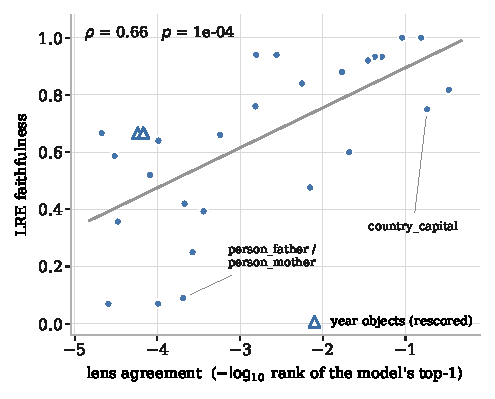
\includegraphics[width=\columnwidth]{fig_lens_vs_faith.pdf}
\caption{LRE faithfulness against the relation-agnostic lens score, 28
relations. The lens sees no relation template, no objects, and no
(subject, object) pairs, and uses one fixed layer throughout.
Triangles mark the two relations with numeric objects, rescored as
described in \S\ref{sec:artifact}.}
\label{fig:main}
\end{figure}

Figure~\ref{fig:main} shows the result. The relation-agnostic score
predicts LRE faithfulness at Spearman $\rho = 0.658$
($p = 1.4\!\times\!10^{-4}$; permutation null $0.0003$ over $10^4$
shuffles).

\paragraph{The correlation is not carried by cardinality.} Relations
differ greatly in how many distinct objects they have; $k$, the mean number
of subjects per object, ranges from $1.0$ to $189$. High $k$ makes
faithfulness easier, and indeed $k$ predicts faithfulness on its own
($\rho = 0.43$, $p = 0.02$). But $k$ is unrelated to the lens score
($\rho = -0.03$, $p = 0.87$), and partialling it out \emph{raises} the
correlation to $\rho = 0.744$ ($p = 10^{-5}$).

\paragraph{Nor by answer frequency.} A relation whose answers are frequent
tokens might be easy for both measures. We estimate the model's prior over
each answer token by averaging its log-probability across ten neutral
contexts. This predicts neither faithfulness ($\rho = -0.03$) nor the lens
score ($\rho = -0.02$), and partialling it out leaves the correlation
unchanged at $0.658$; with both covariates, $0.746$.

\paragraph{Nor by one domain.} Eleven of the 28 relations have
\textit{person} subjects, raising the worry that one domain drives the
result. Holding out each subject domain in turn leaves
$\rho \in [0.570, 0.700]$, median $0.656$.

\paragraph{A within-domain check.} \textsc{person\_father} and
\textsc{person\_mother} are separate relations over near-identical subject
sets. They receive almost identical faithfulness ($0.09$, $0.07$) and
almost identical lens scores ($-3.69$, $-3.99$), without the lens being
told which relation it is looking at.

\section{Where the diagnostic fails}

Two relations sit well above the trend: \textsc{name\_gender}
(faithfulness $0.67$, lens $-4.67$) and \textsc{person\_university}
($0.59$, $-4.52$). Both are cases where the model can answer but a neutral
``known for'' readout has no reason to surface the answer: a first name
does not evoke a gender word, and few people are chiefly known for their
university. This is the diagnostic's main systematic weakness---it
measures what an entity is \emph{salient} for, which is not always what a
relation asks for.

\section{A first-token scoring artifact}
\label{sec:artifact}

Both relations with numeric objects
(\textsc{presidents\_birth\_year}, \textsc{presidents\_election\_year})
initially scored faithfulness $1.000$. This was spurious. In this
tokenizer \texttt{" 1743"} segments as \texttt{[\,' ', '174', '3'\,]}:
digits never merge with a preceding space. First-token scoring therefore
compared the model's top-1 against a bare space token on both sides, and
faithfulness $1.000$ meant only that the LRE and the model both emit a
space.

The fix is to place the space in the prompt, so that the query ends with
it and the next token is content. Rescored, the two relations give
faithfulness $0.67$ and lens scores of $-4.24$ and $-4.17$; the model does
predict the year correctly once the space is consumed. Including the
uncorrected values would have depressed the reported correlation from
$0.658$ to $0.427$.

We flag this because the failure is silent: it produces a perfect score
rather than an obvious error, and it will affect any first-token
evaluation on numeric or unit-prefixed answers.

\section{Limitations}

The study covers one model and 28 relations. The relationship is
correlational: we show that a relation-agnostic readout predicts LRE
faithfulness, not that the representation it reads is what the LRE
exploits: an intervention experiment is the natural next step. Seven of the
28 relations have fewer than ten test items after the in-context and
reference subjects are removed, so their faithfulness estimates are coarse
(for three of them, quantized to thirds); a rotating-split protocol would
sharpen these. Finally, the diagnostic is defined only for relations whose
subjects are entities, which excludes 19 of the dataset's 47 relations.

\section{Conclusion}

Whether a relation is linearly decodable from a language model is
substantially predictable without the relation. A Jacobian lens estimated
from subject differences under a neutral prompt, at a fixed layer, ranks
the model's own answer highly for exactly those relations whose LREs turn
out to be faithful. This locates linear decodability in what a subject's
representation already carries, and suggests that the wide spread of LRE
faithfulness across relations is less about the relations than about the
entities they are asked about.

\bibliography{custom}

\appendix

\section{All relations}

Table~\ref{tab:relations} gives faithfulness and the lens score for every
relation in the study.

\begin{table*}[t]
\centering\footnotesize
\begin{tabular}{@{}lrrr@{\hspace{3em}}lrrr@{}}
\toprule
relation & $k$ & faith. & $A_r$ & relation & $k$ & faith. & $A_r$ \\
\midrule
country\_language$^{*}$ & 1.7 & 1.00 & $-1.04$ & presidents\_election\_year$^{\dagger}$ & 1.1 & 0.67 & $-4.17$ \\
country\_largest\_city$^{*}$ & 1.0 & 1.00 & $-0.81$ & product\_by\_company & 17.4 & 0.66 & $-3.24$ \\
landmark\_on\_continent & 189.4 & 0.94 & $-2.81$ & person\_plays\_position\_in\_sport & 68.0 & 0.64 & $-3.99$ \\
person\_native\_language & 30.6 & 0.94 & $-2.56$ & person\_band\_lead\_singer$^{*}$ & 1.0 & 0.60 & $-1.68$ \\
name\_birthplace & 3.9 & 0.93 & $-1.29$ & person\_university & 1.3 & 0.59 & $-4.52$ \\
name\_religion & 6.2 & 0.93 & $-1.37$ & company\_hq & 4.1 & 0.52 & $-4.09$ \\
person\_plays\_pro\_sport & 63.6 & 0.92 & $-1.45$ & superhero\_person & 1.0 & 0.48 & $-2.15$ \\
person\_plays\_instrument & 85.5 & 0.88 & $-1.77$ & star\_constellation & 11.7 & 0.42 & $-3.67$ \\
landmark\_in\_country & 9.2 & 0.84 & $-2.25$ & pokemon\_evolutions & 1.0 & 0.39 & $-3.44$ \\
city\_in\_country & 1.3 & 0.82 & $-0.48$ & country\_currency & 1.3 & 0.36 & $-4.48$ \\
person\_occupation & 26.5 & 0.76 & $-2.81$ & superhero\_archnemesis & 1.1 & 0.25 & $-3.57$ \\
country\_capital\_city$^{*}$ & 1.0 & 0.75 & $-0.74$ & person\_father & 1.0 & 0.09 & $-3.69$ \\
name\_gender$^{*}$ & 9.5 & 0.67 & $-4.67$ & company\_ceo & 1.0 & 0.07 & $-4.59$ \\
presidents\_birth\_year$^{\dagger}$ & 1.3 & 0.67 & $-4.24$ & person\_mother & 1.0 & 0.07 & $-3.99$ \\
\bottomrule
\end{tabular}
\caption{All 28 relations, sorted by LRE faithfulness. $k$ is the mean number
of subjects per distinct object; $A_r$ is the relation-agnostic lens score, higher
meaning closer agreement with the model. $^{\dagger}$rescored for the
numeric-object artifact (\S\ref{sec:artifact}); $^{*}$fewer than ten test items,
so faithfulness is coarsely quantized.}
\label{tab:relations}
\end{table*}


\end{document}
